%% LyX 2.1.3 created this file.  For more info, see http://www.lyx.org/.
%% Do not edit unless you really know what you are doing.
\documentclass[english]{beamer}
\usepackage{mathptmx}
\usepackage[T1]{fontenc}
\usepackage[latin9]{inputenc}
\usepackage{babel}
\usepackage{url}
\usepackage{amsmath}
\usepackage{amssymb}
\usepackage{graphicx}
\ifx\hypersetup\undefined
  \AtBeginDocument{%
    \hypersetup{unicode=true}
  }
\else
  \hypersetup{unicode=true}
\fi

\makeatletter
%%%%%%%%%%%%%%%%%%%%%%%%%%%%%% Textclass specific LaTeX commands.
 % this default might be overridden by plain title style
 \newcommand\makebeamertitle{\frame{\maketitle}}%
 % (ERT) argument for the TOC
 \AtBeginDocument{%
   \let\origtableofcontents=\tableofcontents
   \def\tableofcontents{\@ifnextchar[{\origtableofcontents}{\gobbletableofcontents}}
   \def\gobbletableofcontents#1{\origtableofcontents}
 }

\@ifundefined{date}{}{\date{}}
%%%%%%%%%%%%%%%%%%%%%%%%%%%%%% User specified LaTeX commands.
\usetheme{Antibes}
\usecolortheme{beaver}
\usefonttheme{default}
\useinnertheme{circles}

\setbeamercovered{transparent}
\setbeamersize{text margin left=0.5cm}
\setbeamertemplate{footline}[frame number]
\setbeamertemplate{navigation symbols}{}

\setbeamersize{text margin left=0.4cm}
\setbeamersize{text margin right=0.4cm}

\usepackage{lmodern}
\usepackage[protrusion=true,expansion=true]{microtype}

\usepackage{color}
\usepackage{listings}
\usepackage{setspace}

\definecolor{Code}{rgb}{0,0,0}
\definecolor{Decorators}{rgb}{0.5,0.5,0.5}
\definecolor{Numbers}{rgb}{0.5,0,0}
\definecolor{MatchingBrackets}{rgb}{0.25,0.5,0.5}
\definecolor{Keywords}{rgb}{0,0,1}
\definecolor{self}{rgb}{0,0,0}
\definecolor{Strings}{rgb}{0,0.63,0}
\definecolor{Comments}{rgb}{0,0.63,1}
\definecolor{Backquotes}{rgb}{0,0,0}
\definecolor{Classname}{rgb}{0,0,0}
\definecolor{FunctionName}{rgb}{0,0,0}
\definecolor{Operators}{rgb}{0,0,0}
\definecolor{Background}{rgb}{0.98,0.98,0.98}

\usepackage{listings}
\lstset{
numbers=left,
numberstyle=\scriptsize,
numbersep=1em,
xleftmargin=1em,
framextopmargin=2em,
framexbottommargin=2em,
showspaces=false,
showtabs=false,
showstringspaces=false,
frame=l,
tabsize=4,
% Basic
basicstyle=\ttfamily\footnotesize\setstretch{1},
backgroundcolor=\color{Background},
language=Python,
% Comments
commentstyle=\color{Comments}\slshape,
% Strings
stringstyle=\color{Strings},
morecomment=[s][\color{Strings}]{"""}{"""},
morecomment=[s][\color{Strings}]{'''}{'''},
% keywords
morekeywords={import,from,class,def,for,while,if,is,in,elif,else,not,and,or,print,break,continue,return,True,False,None,access,as,,del,except,exec,finally,global,import,lambda,pass,print,raise,try,assert,with},
keywordstyle={\color{Keywords}\bfseries},
% additional keywords
morekeywords={[2]@invariant},
keywordstyle={[2]\color{Decorators}\slshape},
emph={self},
emphstyle={\color{self}\slshape},
%
}

\setbeamertemplate{footline}[text line]{%
  \parbox{\linewidth}{\vspace*{-8pt}\href{http://www.czielinski.de/}{\insertshortauthor}\hfill\insertpagenumber}}

\makeatother

\usepackage{listings}
\renewcommand{\lstlistingname}{Listing}

\begin{document}

\title{Concurrent Computations\\
on Multicore Processors}


\subtitle{Threads \& Subprocesses}


\author{Christian Zielinski}


\institute{18\textsuperscript{th}\,June 2015 -- PyCon SG 2015}

\makebeamertitle

\section{Introduction}


\subsection{Introduction}
\begin{frame}{Who am I?}

\begin{itemize}
\item Currently a Ph.D.~student at Nanyang Technological University

\begin{itemize}
\item Working in computational physics, i.e.~simulation of elementary particles
with Monte Carlo methods (``\href{http://en.wikipedia.org/wiki/Lattice_QCD}{lattice quantum chromodynamics}'')
\end{itemize}
\item First experiments with Python around ten years ago
\item Heavy user of Python, \texttt{\textbf{numpy}} and \texttt{\textbf{scipy}}
for data analysis and evaluation of numerical algorithms
\item Slides available on:
\end{itemize}

\begin{center}
\url{www.github.com/czielinski/pyconsg2015}
\par\end{center}

\end{frame}



\subsection{Concurrency}
\begin{frame}{Why concurrency?}

\begin{itemize}
\item Python is \textit{awesome}, but slow

\begin{itemize}
\item C/C++ is typically 10--100 times faster
\end{itemize}
\item Single CPU core performance only improves slowly over time

\begin{itemize}
\item But modern processors have increasing number of cores
\end{itemize}
\item Blocking operations like I/O cause idle time

\begin{itemize}
\item Rather do computations in the meantime
\end{itemize}
\item Concurrency helps to mitigate all problems

\begin{itemize}
\item Potentially significant speed ups
\end{itemize}
\end{itemize}
\end{frame}

\begin{frame}{Concurrency in Python}

\begin{itemize}
\item How to make us of concurrency in Python?
\item For stock Python typically use either

\begin{itemize}
\item Threads via the \texttt{\textbf{threading}} module
\item Subprocesses via the \texttt{\textbf{multiprocessing}} module
\end{itemize}
\item They provide convenient high-level interfaces

\begin{itemize}
\item \texttt{\textbf{threading}} and \texttt{\textbf{multiprocessing}}
have similar API
\end{itemize}
\item There are great third-party modules to go beyond a single CPU:

\begin{itemize}
\item \texttt{\textbf{mpi4py}}, \texttt{\textbf{pycuda}}, \texttt{\textbf{pyopencl}}
(but not today's topic)
\end{itemize}
\end{itemize}
\end{frame}

\begin{frame}{Global Interpreter Lock (GIL)}

\begin{itemize}
\item CPython's threads are real POSIX / Windows threads
\item The Global Interpreter Lock (GIL) prevents that more than one thread
is executing Python bytecode at the same time
\item The Global Interpreter Lock:

\begin{itemize}
\item makes the CPython interpreter explicitly thread-safe
\item simplifies CPython's code base
\item prevents true parallel threading
\item is released during I/O
\end{itemize}
\item The GIL is implementation dependent

\begin{itemize}
\item CPython and PyPy have a GIL
\item Jython and IronPython have no GIL
\end{itemize}
\end{itemize}
\end{frame}



\section{Overview}


\subsection{Threads}
\begin{frame}{Threads}

\begin{itemize}
\item Threads are accessible via \texttt{\textbf{threading}} module

\begin{itemize}
\item Can be spawned quickly
\item Share memory
\end{itemize}
\item Threads can be useful for I/O bound problems

\begin{itemize}
\item Do useful operations during blocking operations
\end{itemize}
\item Usually not suited for CPU bound problems

\begin{itemize}
\item GIL prevents true parallel computations\\
(with a few exceptions, e.g.~some \texttt{\textbf{numpy}} functions)
\item Introduce additional overhead
\end{itemize}
\item Use \texttt{\textbf{Lock}} to define critical sections,\\
i.e.~code that requires mutual exclusion of access
\end{itemize}
\end{frame}

\begin{frame}[fragile]{Simple threading example}




\begin{lstlisting}
import threading as th

def worker(lock, num):
  cubed = num**3
  # A worker should actually avoid I/O ...
  lock.acquire()
  print("{} cubed is {}".format(num, cubed))
  lock.release()

my_threads = []
for i in range(4):
  lock = th.Lock()
  t = th.Thread(target=worker, args=(lock, i))
  my_threads.append(t)
  t.start()
\end{lstlisting}

\end{frame}



\subsection{Subprocesses}
\begin{frame}{Subprocesses (I)}



\begin{itemize}
\item Subprocesses accessible via \texttt{\textbf{multiprocessing}} module

\begin{itemize}
\item Self-sufficient interpreter instance
\item No memory sharing
\end{itemize}
\item Subprocesses have their own interpreter instance

\begin{itemize}
\item Spawning takes long time, significant overhead
\item Every subprocess has own GIL, allow for true parallelism
\end{itemize}
\end{itemize}
\end{frame}

\begin{frame}{Subprocesses (II)}

\begin{itemize}
\item Subprocesses suited for CPU bound problems

\begin{itemize}
\item Can do computations truly in parallel to utilize several cores
\item Usually not useful to spawn more than one subprocess per \textit{physical}
core
\end{itemize}
\item Not suited for I/O bound problems

\begin{itemize}
\item Cannot e.g.~read files faster from HDD
\item To keep cores busy need to feed data quickly enough
\item Potential memory bandwidth bottleneck for large number of cores
\end{itemize}
\end{itemize}
\end{frame}

\begin{frame}[fragile]{Simple multiprocessing example}




\begin{lstlisting}
import multiprocessing as mp

def worker(lock, num):
  cubed = num**3
  # A worker should actually avoid I/O ...
  lock.acquire()
  print("{} cubed is {}".format(num, cubed))
  lock.release()

my_procs = []
for i in range(4):
  lock = mp.Lock()
  p = mp.Process(target=worker, args=(lock, i))
  my_procs.append(p)
  p.start()
\end{lstlisting}

\end{frame}



\subsection{Theory}
\begin{frame}{Scaling and Amdahl's law}

\begin{itemize}
\item Using $N$ cores does not automatically reduce runtime by a factor
of $N$

\begin{itemize}
\item Some code section inherently serial, like I/O
\item Some algorithms are difficult to parallelize, e.g.~recursive functions
\item One usually parallelizes only the performance-critical parts of the
code
\end{itemize}
\item \href{http://dl.acm.org/citation.cfm?doid=1465482.1465560}{Amdahl's law}
{[}Amdahl '67{]}

\begin{itemize}
\item Parallelizing a program with serial runtime $T\left(1\right)$ with
$N$ processes and serial code fraction $f\in\left[0,1\right]$ results
in runtime:
\[
T\left(N\right)=T\left(1\right)\cdot\left(f+\frac{1}{N}\left(1-f\right)\right)
\]

\item So for sufficiently large $N$ runtime is dominated by serial code
sections!
\end{itemize}
\end{itemize}
\end{frame}

\begin{frame}


\begin{figure}
\begin{centering}
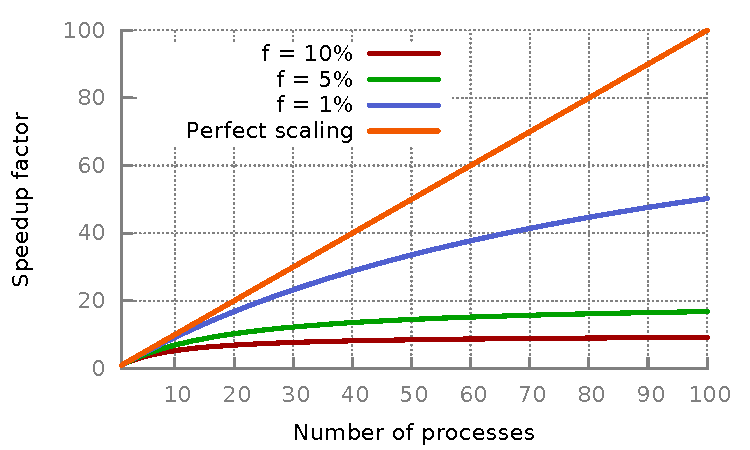
\includegraphics[width=1\columnwidth]{images/amdahl}
\par\end{centering}

\protect\caption{Amdahl's law}
\end{figure}


\end{frame}

\begin{frame}{Some general remarks}

\begin{itemize}
\item Split up larger problems into smaller subproblems with appropriate
size

\begin{itemize}
\item If too small, performance degraded due to overhead
\item If too large, load balancing becomes problematic
\end{itemize}
\item Many methods are not thread-safe

\begin{itemize}
\item Use \texttt{\textbf{Lock.acquire()}} and \texttt{\textbf{Lock.release()}}
in critical code sections
\item Note: even \texttt{\textbf{print}} is not thread-safe
\end{itemize}
\item Arguing about the correctness of a parallel program is hard

\begin{itemize}
\item Order of computations are not fixed
\end{itemize}
\end{itemize}
\end{frame}



\section{Multiprocessing API}
\begin{frame}


\begin{center}
{\LARGE{}API of the }\texttt{\textbf{\LARGE{}multiprocessing}}{\LARGE{}
module}
\par\end{center}{\LARGE \par}

\end{frame}



\subsection{Worker pools}
\begin{frame}{Worker pools}

\begin{itemize}
\item Simplest parallelization strategy is to use a worker pool

\begin{itemize}
\item Accessible via \texttt{\textbf{multiprocessing.Pool}}
\end{itemize}
\item Important methods:

\begin{itemize}
\item \texttt{\textbf{map}} (\texttt{\textbf{map\_async}}) for (asynchronous)
parallel map
\item \texttt{\textbf{apply\_async}} for asynchronous function evaluation
\end{itemize}
\item Limitations:

\begin{itemize}
\item Can only deal with pickable objects
\item Cannot use \texttt{\textbf{lambda}} expressions, nested functions,
class methods
\item Can use global functions, global classes and partial functions via
\texttt{\textbf{functools.partial}}
\item \texttt{\textbf{Pool}} will not work in interactive sessions\\
(\texttt{\textbf{\_\_main\_\_}} module has to be importable by the
children)
\end{itemize}
\end{itemize}
\end{frame}

\begin{frame}[fragile]{Parallel map}


\begin{lstlisting}
from multiprocessing import Pool

def cube(num):
  return num**3

if __name__ == '__main__':
  # Can also specify 'processes' parameter
  p = Pool()
  # Equivalent of serial map(cube, range(10))
  res = p.map(cube, range(10))
  print(res)
  # Output: [0, 1, 8, 27, 64, 125, 216, 343, 512, 729]
\end{lstlisting}
Note: This overly simplified example runs slower than the serial version

\end{frame}

\begin{frame}[fragile]{Asynchronous function evaluation}


\begin{lstlisting}
from multiprocessing import Pool

def double(arg):
  return 2*arg

def cube(num):
  return num**3

if __name__ == '__main__':
  p = Pool()
  f1_get = p.apply_async(cube, args=(6,))
  f2_get = p.apply_async(double, args=('haha',))
  # Do other work here
  res = [f1_get.get(), f2_get.get()]
  print(res)
  # Output: [216, 'hahahaha']
\end{lstlisting}


\end{frame}



\subsection{Sharing data}
\begin{frame}


\begin{center}
{\LARGE{}Sharing data}
\par\end{center}{\LARGE \par}

\end{frame}

\begin{frame}[fragile]{Shared memory maps}


To share state with a \texttt{\textbf{Process}} use shared memory
maps:\\
\begin{lstlisting}
from multiprocessing import Process, Array

def cube_arr(arr):
  for i in range(len(arr)):
    arr[i] = arr[i]**3

if __name__ == '__main__':
  shared_arr = Array('i', range(10))  # 'd' for double
  p = Process(target=cube_arr, args=(shared_arr,))
  p.start()
  # Do other work here
  p.join()
  print(shared_arr[:])  
  # Output: [0, 1, 8, 27, 64, 125, 216, 343, 512, 729]
\end{lstlisting}


\end{frame}

\begin{frame}[fragile]{Server processes and managers}


Alternatively use a \texttt{\textbf{Manager}} for more complex objects:\\
\begin{lstlisting}
from multiprocessing import Process, Manager

def modify_names(names):
  names['Alice'] = 42
  if 'Bob' in names:
    shared_dict['Bob'] += 1

if __name__ == '__main__':
  with Manager() as m:
    shared_dict = m.dict()
    shared_dict['Bob'] = 7
    p = Process(target=modify_names, args=(shared_dict,))
    p.start()
    # Do other work here
    p.join()
    print(shared_dict)  # Output: {'Bob': 8, 'Alice': 42}
\end{lstlisting}


\end{frame}



\subsection{Interprocess communication}
\begin{frame}


\begin{center}
{\LARGE{}Interprocess communication}
\par\end{center}{\LARGE \par}

\end{frame}

\begin{frame}[fragile]{Pipes}


To communicate between two processes use a \texttt{\textbf{Pipe}}:\\
\begin{lstlisting}
from multiprocessing import Process, Pipe

def cube(my_pipe):
  data = my_pipe.recv()
  my_pipe.send([n**3 for n in data])

if __name__ == '__main__':
  parent_pipe, child_pipe = Pipe()
  p = Process(target=cube, args=(child_pipe,))
  p.start()
  parent_pipe.send(range(10))  # Send work
  # Do other work here
  print(parent_pipe.recv())
  p.join()
  # Output: [0, 1, 8, 27, 64, 125, 216, 343, 512, 729]
\end{lstlisting}


\end{frame}

\begin{frame}[fragile]{Queues}


For several processes can use a \texttt{\textbf{Queue}}:\\
\begin{lstlisting}
from multiprocessing import Process, Queue

def place_work(q):
  q.put(range(10))

def process_work(q):
  data = q.get()
  q.put([n**3 for n in data])

if __name__ == '__main__':
  queue = Queue()
  p1 = Process(target=place_work, args=(queue,))
  p2 = Process(target=process_work, args=(queue,))
  p1.start(); p2.start()  # Now do other work
  p1.join(); p2.join()
  print(queue.get())  # Output: [1, 64, 343]
\end{lstlisting}


\end{frame}



\subsection{Guidelines}
\begin{frame}{Guidelines (I)}

\begin{itemize}
\item Most important: Only parallelize where necessary!
\item Try to avoid sharing state if possible
\item If need to share:

\begin{itemize}
\item Use \texttt{\textbf{Value}} and \texttt{\textbf{Array}} for simple
data
\item Use server process \texttt{\textbf{Manager}} for more complex objects
\end{itemize}
\item For interprocess communication use \texttt{\textbf{Pipe}} and \texttt{\textbf{Queue}}

\begin{itemize}
\item Pipes for fast point-to-point communication
\item Queues are multi-producer, multi-consumer FIFO queues
\end{itemize}
\end{itemize}
\end{frame}

\begin{frame}{Guidelines (II)}

\begin{itemize}
\item Explicitly pass resources to subprocesses and avoid global variables
as they can lead to inconsistencies (Windows)
\item Ensure that the main module can be safely imported by a new Python
instance (Windows)

\begin{itemize}
\item Use \texttt{\textbf{if \_\_name\_\_ == '\_\_main\_\_'}} guard to avoid
side effects
\end{itemize}
\item Avoid \texttt{\textbf{Process.terminate}} as it might break access
to shared resources
\item Read more on:\\
\texttt{\textbf{\scriptsize{}\href{https://docs.python.org/2/library/multiprocessing.html\#programming-guidelines}{https://docs.python.org/2/library/multiprocessing.html\#{}programming-guidelines}}}{\scriptsize \par}
\end{itemize}
\end{frame}



\subsection{Demo}
\begin{frame}{{\LARGE{}Time for a short demo!}}

\begin{itemize}
\item Midpoint rule for numerical integration
\[
\intop_{a}^{b}f\left(x\right)\,\mathsf{d}x\approx h\sum_{k=1}^{N}f\left(a+\left(k-\frac{1}{2}\right)h\right),\qquad h=\frac{b-a}{N}
\]

\item Allows for straightforward parallel evaluation
\[
\intop_{a}^{b}f\left(x\right)\,\mathsf{d}x=\intop_{a}^{c}f\left(x\right)\,\mathsf{d}x+\intop_{c}^{b}f\left(x\right)\,\mathsf{d}x,\qquad\forall c\in\mathbb{R}
\]

\item Can split up large integration range into several small ones, which
can be evaluated in parallel
\end{itemize}



\end{frame}



\subsection{Questions \& Answers}
\begin{frame}


\begin{center}
{\LARGE{}Questions \& Answers}\\
(if time permits)\bigskip{}

\par\end{center}


\begin{center}
Slides on:\\
\texttt{\textbf{\url{www.github.com/czielinski/pyconsg2015}}}
\par\end{center}


\end{frame}

\end{document}
